\section{Methodology}\label{sec:Methodology}

% O desenvolvimento do SISDOT deu-se no âmbito do projeto PROMISE-EB (Projeto de Pesquisa para Validação de Práticas e Métodos de Desenvolvimento de Software para o Exército Brasileiro). Entre as atividades deste projeto estava o desenvolvimento do SISDOT, a partir de um sistema já existente, escrito na linguagem Delphi e voltado para o ambiente desktop.

The development of SISDOT took place within the scope of the project PROMISE-EB (Project of Research for Validation of Practices and Methods of Software Development for the Brazilian Army). Among the activities of this project was the development of SISDOT, from an existing system, written in the Delphi language and aimed at the desktop environment.

% Como não foi possível utilizar o sistema legado, foi realizada uma engenharia reversa a partir do manual do usuário deste sistema, já que sistemas legados costumam ser uma das fontes de informação essenciais para a análise de domínio de aplicações. Além disso, foi realizado diversas interações com os usuários do sistema, os quais possuiam um domínio abrangente do sistema legado. A Engenharia de Domínio (ED) se preocupa com a identificação e modelagem de características comuns e variáveis em aplicações de um dado domínio, gerando como resultado modelos de domínio (por exemplo, casos de uso de domínio, classes do domínio e etc.), com o apoio oferecido por processos de ED que, geralmente, compreendem as fases de análise, projeto e implementação foi possível identificar as funcionalidades e regras de negócio do sistema legado (SISDOT).

As it was not possible to use the legacy system, reverse engineering was done from the user manual of this system, since legacy systems are often one of the essential sources of information for the application domain analysis. Furthermore, a number of interactions were made with the users of the system, which had a comprehensive domain of the legacy system. Domain Engineering (ED) is concerned with the identification and modeling of common and variable characteristics in applications of a given domain, resulting in domain models (for example, domain use cases, domain classes and etc.) with the support offered by ED processes that generally comprise the phases of analysis, design and implementation, it was possible to identify the functionalities and business rules of the legacy system (SISDOT).

% O desenvolvimento do sistema foi baseado no processo de desenvolvimento ágil, onde em cada sprint eram realizadas as fases de análise, projeto, implementação, teste e implantação. Na fase de análise foi realizado o levantamento de requisitos a partir das informações contidas no manual de uso do sistema legado e complementadas pelos usuários do sistema. Na fase de projeto os modelos de análise foram refinados visando a construção ou adaptação da arquitetura do domínio. Os modelos da fase de projeto quase sempre eram informais, exceto em alguns casos mais complicados, com a intenção de dar uma visão geral do que deveria ser desenvolvido em determinado sprint. Na fase de implementação foram escritos os códigos necessários, juntamente com seus casos de teste. Ao fim do sprint era realizada a implantação no ambiente de homologação, permitindo a utilização por parte dos usuários e seus respectivos feedbacks. Essas iterações permitiram o refinamento das funcionalidades e as possíveis alterações necessárias para a execução das funcionalidades.

The development of the system was based on the agile development process, where in each sprint the phases of analysis, design, implementation, testing and deployment were performed. In the analysis phase, requirements were surveyed based on the information contained in the legacy system user manual and complemented by the users of the system. In the design phase the analysis models were refined aiming at the construction or adaptation of the architecture of the domain. The design phase models were almost always informal, except in some cases more complicated, with the intention of giving an overview of what should be developed in a given sprint. In the implementation phase the necessary codes were written along with their test cases. At the end of the sprint, the deployment was carried out in the homologation environment, allowing the users to use and their respective feedbacks. These iterations allowed the refinement of the functionalities and the possible changes necessary for the execution of the functionalities.

% Durante a modelagem das entidades referentes ao domínio da high level rule, foi identificada a semelhança entre a definição de um high level rule e uma regra do tipo ``se-então''. Como os high level rules servem de base para a geração de QDMs foi identificado que estes poderiam ser gerados automaticamente por um rule engine, a partir de um conjunto de regras ``se-então'', os high level rule. Com isso, foi então escolhido o Drools como rule engine, uma vez que: a equipe já possuia conhecimento sobre a ferramenta, a existência de uma linguagem que permitiria a conversão, com facilidade, de high level rule para esta linguagem, vasta documentação e uma comunidade expressiva, além de ser desenvolvida por uma empresa conceituada no mundo do desenvolvimento de software, a RedHat, hoje parte da IBM.

During the modeling of entities related to the high level rule domain, the similarity between the definition of a high level rule and a ``if-then'' rule was identified. As high level rules serve as a basis for the generation of QDMs, it has been identified that they could be generated automatically by a rule engine, from a set of ``if-then'' rules, the high level rule. Based on that, Drools was chosen as a rule engine, since: the team already had knowledge about the tool, the existence of a language that would allow the conversion, with ease, of high level rule for this language, extensive documentation and a expressive community, in addition to being developed by a reputed company in the world of software development, RedHat, now part of IBM.

% Os testes iniciais para a geração de QDMs exigiam a declaração de high level rule na linguagem Java, o que era, na maioria dos casos, muito moroso, exigindo dezenas de linhas de código, mesmo utilizando alguns métodos auxiliares que aumentavam o reuso. Além disso, a definição do resultado esperado, para comparar com o QDM gerado, necessitava da presença do usuário, para indicar/verificar os resultados reais. Quando não era possível a presença do usuário, o testador devia analisar manualmente o QC para identificar os resultados esperados, e declará-los utilizando a linguagem Java para a conferência no final da execução dos testes. Estes foram os fatores essenciais que levaram ao desenvolvimento de uma DSL, que visava facilitar a declaração de high level rule, e do uso da ferramenta cucumber para a definição de casos de teste. Apesar disso, os testes ainda eram definidos de forma manual, embora já houvesse um ganho expressivo de produtividade, e ainda necessitavam do usuário ou de uma análise do QC para definição dos resultados esperados. Assim, foi desenvolvida uma solução para a geração automática de testes e para a geração de QDMs, onde eram gerados automaticamente tanto o high level rule quanto o resultado esperado, assim como a definição do caso de teste em cucumber.

The initial tests for generating QDMs required the declaration of high level rule in the Java language, which was, in most cases, very time-consuming, requiring dozens of lines of code, even using some auxiliary methods that increased reuse. Furthermore, the definition of the expected result, to compare with the generated QDM, required the presence of the user to indicate/verify the actual results. When user presence was not possible, the tester should manually analyze the QC to identify expected results, and declare them using the Java language for the conference at the end of the test run. These were the key factors that led to the development of a DSL, which aimed to facilitate the declaration of high level rule, and the use of the cucumber tool for the definition of test cases. Despite this, the tests were still manually defined, although there was already an expressive gain in productivity, and they still needed the user or a QC analysis to define the expected results. Thus, a solution was developed for the automatic generation of tests and for the generation of QDMs, where both the high level rule and the expected result were generated automatically, as well as the definition of the test case in cucumber.

\begin{figure}[!ht] %\centering
	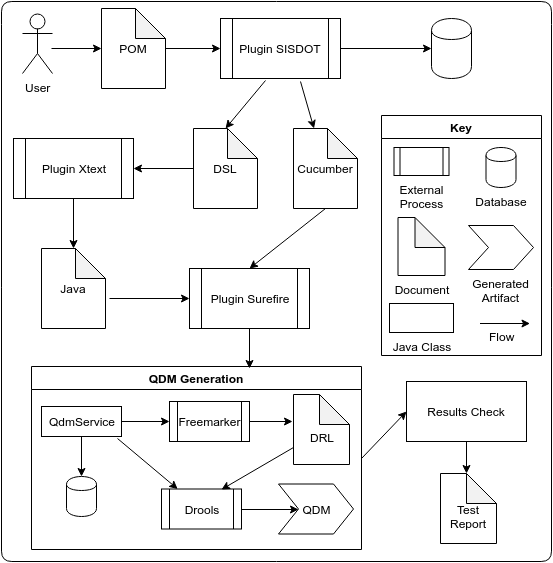
\includegraphics[scale=0.40]{img/processo.png}
	\caption{Tests Generation Process} 
	\label{fig:process}
\end{figure}
